\documentclass{article}
\usepackage{graphicx}

\begin{document}

\title{Software Construction HW1}
\author{William Horn\\University of Alaska Fairbanks\\wbhorn@alaska.edu}
\date{\today}
\maketitle

\section{Gitting Started}
\textbf{Repository URL}: https://github.com/williamh890/cs372-hw1 \\

\begin{figure}[h!]
  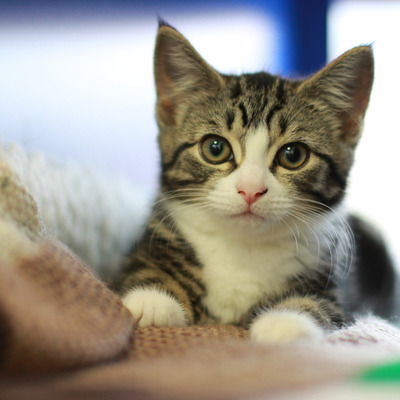
\includegraphics[width=\linewidth]{cat.jpg}
  \caption{A cute cate.}
  \label{fig:cat1}
\end{figure}

\section{Useful Git Commands}
\subsection{git stash}
Git stash allows you to temporarily save your work onto a stack and pop the changes off whenever you like.
This is super useful when you want to pull but don't yet want to commit your changes. You can run a 'git stash' pull
down the changes then run 'git stash pop' to merge the changes you stash back in without ever committing.
\subsection{git diff}
This command allows you to quickly see the differences in your code. Without any arguments it compares unstated changes
with the previous commits, but can be used to compare between commits also.
\subsection{git reset --hard}
I use this when I just don't care about the changes I just made. This is a quick and dirty way to
get back to the previous commits. Be careful however, with greate power, comes greate responsibility.
Make extra sure you don't want the current changes because after running this command, they are gone.

\end{document}
